\section{Cross-Site Scripting (XSS)}
Beim Cross-Site Scripting schleust der Angreifer Skriptcode in dynamisch erstellte Teile von Webseiten ein. Viele glauben dass damit nur nervige Nachrichtenboxen oder \"ahnliche Effekte hervorgerufen werden k\"onnen. Dies entspricht jedoch absolut nicht der Realit\"at. XSS hat wesentlich h\"oheres Potential, welches bis zum Diebstahl von Daten oder das Ver\"andern der Benutzeroberf\"ache. Dass praktisch jede, nicht explizit gesicherte Webseite angreifbar ist, tr\"agt au{\ss}erdem zu dem hohen Gefahrenpotential dieser Attacke bei.\cite{xssBuch}

\subsection{Typen}
Es gibt drei grundlegende Typen von XSS. Diese werden im nachfolgenden kurz erl\"autert:

\begin{itemize}
\item Reflektiertes XSS\\\\
Beim reflektierten XSS wird der zu verwendende Schadcode direkt mit dem Aufruf \"ubergeben. Dies geschieht zum Beispiel durch einer pr\"aparierte URL, welche den Code enth\"alt. Die Verbreitung dieser URL kann \"uber beliebige Wege erfolgen, etwa per Email oder Foreneintr\"age. Das Opfer muss nun nur noch auf den pr\"aparierten Link klicken, dass die Website von dessen Browser inklusive dem eingeschleusten Script Code abgearbeitet wird. Dies ist die am weitesten verbreitete Art dieser Attacke.\\
\item Persistentes XSS\\\\
Bei dieser Art wird der Schadcode in der Datenbank der angegriffenen Website gespeichert. Dies geschieht beispielsweise indem ein Eintrag, welcher Scriptcode enth\"alt in ein Forum gepostet wird. Dieses Forum sendet den Beitrag mit eingebettetem Script nun zu jedem Besucher, der dieses \"offnet. Das Schadenspotential dieser Art ist deutlich h\"oher, da kein Zutun des Opfers notwendig ist, allerdings auch nicht so weit verbreitet wie das reflektierte XSS.\\
\item DOM XSS\\\\
Diese Art ist die am wenigsten verbreitete, da sie von vielen Angreifern als auch potentiellen Opfer-Webseiten oft untersch\"atzt wird. Auch hier wird eine pr\"aparierte URL verwendet. Das in der URL angeh\"angte Script wird nun vom Browser per JavaScript in das eigentlich aufgerufene HTML File eingebunden. Diese Attacke funktioniert aber nur in Browsern welche Sonderzeichen in URLs nicht verarbeiten. Deshalb ist diese Attacke z.B. in Firefox nicht m\"oglich.
\end{itemize}
\cite{xssBuch}

\subsection{Effekte}
Wie schon in der Einleitung zu XSS beschrieben, l\"asst sich wesentlich mehr anstellen als nur l\"astige Mitteilungsboxen darzustellen. Im folgenden werden die m\"oglichen Effekte durch eine XSS Attacke erl\"autert.
\cite{xssBuch}

\subsubsection{Auslesen von Cookies}
Viele Websites speichern wichtige Daten wie zum Beispiel Session IDs in Cookies ab um sp\"ater darauf zugreifen zu k\"onnen und beispielsweise einen eingeloggten Benutzer wiederzuerkennen. Gelingt es, ein derartiges Session Cookie zu stehlen, ist es oft m\"oglich die Sitzung des Besitzers dieses Cookies zu \"ubernehmen. Nun kann mit s\"amtlichen Berechtigungen dieses Nutzers gearbeitet werden, ohne sein Passwort stehlen zu m\"ussen und oft auch ohne dass dieser etwas davon bemerkt.\\
Heutzutage werden Session IDs in Cookies allerdings oft verschl\"usselt, was ein Abh\"oren sehr schwierig macht. XSS kann diese Schutzmechanismen allerdings umgehen, da der Code im Browser des Opfers ausgef\"uhrt wird und daher alle Daten im Klartext vorliegen.
\cite{xssBuch}

\subsubsection{Auslesen von Inhalten der Web Application}
Neben Cookies, kann nat\"urlich auch die aufgerufene Website an sich ausgelesen werden. Dies ist beispielsweise in einem Online Shop relevant, wo am Ende der Bestellung nochmal alle vom Kunden eingegebenen Daten angezeigt werden. Dort angezeigte Kreditkartendaten oder \"ahnliches k\"onnen nun vom Angreifer abgezweigt werden.
\cite{xssBuch}

\subsubsection{\"Ubertragen der Daten an den Angreifer}
Gesammelte Daten m\"ussen auch wieder zum Angreifer \"ubertragen werden k\"onnen. Dies kann durch einen Web Server geschehen, welcher sich im Besitz des Angreifers befindet. Die Per XSS ausgelesenen Daten werden nun in Form einer ung\"ultigen Anfrage an den Server gesandt. Es wird also beispielsweise ein Bild mithilfe des ``<img>'' Tags angefragt, welches nicht existiert. In diese Anfrage werden die vom Opfer extrahierten Daten angeh\"angt sodass sie \"uber das ``access\_log'' File des Webservers ausgelesen werden k\"onnen. Praktischerweise enth\"alt das Log File auch noch zus\"atzliche Informationen wie IP Adresse es Opfers und \"ahnliches.
\cite{xssBuch}

\clearpage
\subsection{Vermeintliche Schutzmechanismen}
Es gibt einige Gegenma{\ss}nahmen, welche oft eine sehr einfache Struktur haben, aber nicht genug Schutz gegen derartige Angriffe bieten.\\
\begin{itemize}
\item Filtern von ``<script></script>'' Tags\\\\
Das Filtern von Script Tags scheint verlockend, da diese dem Browser den Einsatz einer Scriptsprache anzeigen.\\
\item Begrenzen von erlaubten Sonderzeichen\\\\
Auch diese Technik klingt vorerst sehr effektiv, da spezielle Sonderzeichen wie etwa spitze Klammern (``<'' und ``>'') ausgefiltert werden und so auch unterschiedliche Schreibweisen wie ``<sCrIpT>'' unbrauchbar werden.\\
\item Begrenzen der Zeichenanzahl\\\\
Das Begrenzen der Zeichenanzahl h\"atte zus\"atzlich zur Folge, dass nur noch wesentlich simplere Scripte, welche weniger Schaden anrichten eingeschleust werden k\"onnen.\\
\end{itemize}

Alle bisher genannten Schutzmechanismen sehen auf den ersten Blick nach brauchbarem Schutz mit wenig Aufwand aus. Leider k\"onnen sie aber mit mehr oder weniger Aufwand umgangen werden. Es sind zum Beispiel in modernen Browsern oft keine ``<script>'' Tags mehr notwendig, dass JavaScript Code ausgef\"uhrt wird. Es gibt einige Ans\"atze um diese Tags zu umgehen.
\cite{xssBuch}

\clearpage
\subsection{Escapen und listen-basierte Filter}
\subsubsection{Escapen von Sonderzeichen}
Wenn die M\"oglichkeit, Code in bestehende Tags einzuf\"ugen nicht existiert, m\"ussen eigene Tags geschaffen werden. Wie bereits vorher erw\"ahnt, ist das simple Filtern von Tags nicht ausreichend. Mithilfe von Escapen kann man allerdings wesentlich geschickter an die Sache herangehen. Im folgenden werden die Sonderzeichen mit ihren Escape Sequenzen gegen\"ubergestellt.\\
\begin{table}[H]
\centering
\begin{tabular}{|l|l|}
\hline Zeichen & Escape Sequenz \\ 
\hline < & \&lt; \\ 
\hline > & \&gt; \\ 
\hline = & \&equals; \\ 
\hline \& & \&amp; \\ 
\hline \# & \&num; \\ 
\hline + & \&plus; \\ 
\hline - & \&hyphen; \\ 
\hline / & \&sol; \\ 
\hline ? & \&quest; \\ 
\hline ( & \&lpar \\ 
\hline ) & \&rpar \\ 
\hline {\{} & \&lcub; \\ 
\hline {\}} & \&rcub; \\ 
\hline {\$} & \&dollar; \\ 
\hline @ & \&commat; \\ 
\hline \textasciicircum & \&caret; \\ 
\hline * & \&ast; \\ 
\hline : & \&colon; \\ 
\hline ; & \&semi; \\ 
\hline 
\end{tabular} 
\caption{Escape-Sequenzen \cite{xssBuch}}
\label{escape-sequenzen}
\end{table}

W\"ahrend nun ein ``<script src = script.js>'' noch zum Ausf\"uhren des an dieser Stelle geladenen Scripts f\"uhrt, wir ein escaptes ``\&lt;script src \&equals; script.js\&gt;'' nur noch als harmloser Text im Browser angezeigt.
\cite{xssBuch}

\clearpage
\subsubsection{Erkennen von Scripten mithilfe von Listen}
Eine derartige ``Blacklist'' von sch\"adlichen Scripten ist ein sehr hoher Aufwand, da der Ersteller der Liste \"uber sehr viel Fachwissen und verschiedenste Angriffsarten und -vektoren verf\"ugen muss. Aus diesem Grund fertigt ein Web-Entwickler eine solche Liste nicht selbst, sondern beschafft diese von externen Personen oder Organisationen. Ein Beispiel w\"are das Projekt ``safehtml'' welches in der Vergangenheit einen hohen Bekanntheitsgrad erreicht hat, aber leider seit einiger Zeit nicht mehr weitergef\"uhrt wird. Blacklisten haben aber naturgegebene Schwachstellen wie etwa die Unvollst\"andigkeit, man kann nie wissen ob die verwendete Liste bereits die neuesten Sicherheitsrisiken beinhaltet oder hinterherhinkt.
\cite{xssBuch}

\subsubsection{Escapen vs. Listenbasiert}
Prinzipiell ist das Escapen von Inputs vorzuziehen, da es sich in der Praxis als sehr belastbar erwiesen hat und nicht \"uber die bekannten Sch\"achen von Blacklists verf\"ugt. Allerdings gibt es F\"alle wo das Escapen nicht zielf\"uhrend ist. Wenn beispielsweise bei einer Webanwendung wie einem Webmail Client diverse HTML Tags gebraucht werden, kann man diese nicht einfach escapen, da sonst m\"oglicherweise die Formatierung von Emails vernichtet w\"urde. Auch wenn eine bestehende Web Applikation gegen XSS Attacken gesichert werden soll ist es manchmal sinnvoller auf Listen zu setzten. Ein re-design von Input Elementen greift tief in die Struktur einer Applikation ein und Formatierungen von Texten werden m\"oglicherweise unm\"oglich gemacht. Da dies sehr Zeit- und Kostenintensiv sein kann, ist es manchmal sinnvoller auf Listenbasierte Mechanismen zur\"uckzugreifen. Diese reichen zwar nicht an die Sicherheitsstandards von Escapen heran, allerdings kann damit doch schnelle und bis zu einem gewissen Grad ausreichende Abhilfe geschafft werden.
\cite{xssBuch}

\clearpage
\subsection{Beispiel}
\textbf{Hier ein Beispiel eines sehr simplen XSS Angriffs.}\\\\
Eine normale Suchanfrage.
\begin{figure}[H]
	\begin{center}
		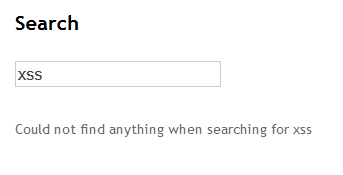
\includegraphics[width=0.3\linewidth]{images/xss1.png}
		\caption{Suchanfrage}
		\label{titel}
	\end{center}
\end{figure}

Das selbe Suchfeld mit injectetem Code.
\begin{figure}[H]
	\begin{center}
		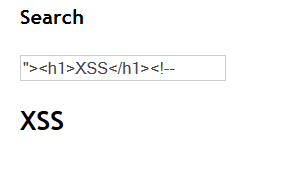
\includegraphics[width=0.3\linewidth]{images/xss2.png}
		\caption{XSS}
		\label{titel}
	\end{center}
\end{figure}
Die Eingabe wird vorzeitig beendet, anschlie{\ss}end der eigene Code eingef\"ugt und der nachfolgende HTML Code der Website auskommentiert. Daher wird auch die eigentliche Meldung der Suche nicht mehr angezeigt.
